\newcommand{\empt}[2]{$#1^{\langle #2 \rangle}$}
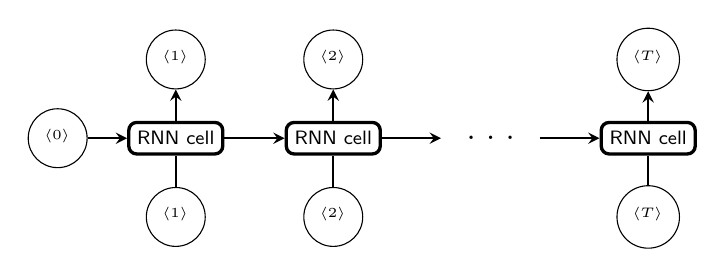
\begin{tikzpicture}[x=1cm, y=1cm, >=stealth, font=\sffamily\scriptsize]
    \tikzstyle{neuron}=[circle, draw, minimum size=.6cm]
    \tikzstyle{dots}=[draw=none, scale=2, text height=0.333cm, execute at begin node={\color{black}\tiny$\cdots$}]
    \tikzstyle{Arrow}=[rounded corners=.20cm,thick] % Arrows with rounded corners
    \tikzstyle{cell}=[% For the main box
        rectangle,
        draw,
        rounded corners=1mm,
        very thick,
        minimum width=6mm,
        minimum height=4mm,
        inner sep=3pt
        ]
    
    % Input nodes
    \node [neuron] (input1) at (0,0) {\empt{\x}{1}};
    \node [neuron] (input2) at (2,0) {\empt{\x}{2}};
    \node [neuron] (inputT) at (6,0) {\empt{\x}{T}};
    
    % Recurrent cells
    \node [cell] (cell1) at (0,1) {RNN cell};
    \node [cell] (cell2) at (2,1) {RNN cell};
    \node [cell] (cellT) at (6,1) {RNN cell};
    
    % Hidden nodes
    \node [neuron] (hidden0) at (-1.5,1) {\empt{\h}{0}};
    \node [neuron] (hidden1) at (0,2) {\empt{\h}{1}};
    \node [neuron] (hidden2) at (2,2) {\empt{\h}{2}};
    \node [neuron] (hiddenT) at (6,2) {\empt{\h}{T}};
    
    % Dots
    \node [neuron, draw=none, scale=2] (dots1) at (4,1) {\tiny$\dots$};
    
    % Hidden to cell to cell ... to cell
    \draw [->, Arrow] (hidden0) -- (cell1);
    \draw [->, Arrow] (cell1) -- (cell2);
    \draw [->, Arrow] (cell2) -- (dots1);
    \draw [->, Arrow] (dots1) -- (cellT);
    
    % Input to cell to hidden
    \draw [->, Arrow] (input1) -> (cell1) -- (hidden1);
    \draw [->, Arrow] (input2) -> (cell2) -- (hidden2);
    \draw [->, Arrow] (inputT) -> (cellT) -- (hiddenT);
\end{tikzpicture}